%%
%% This is file `sample-sigconf.tex',
%% generated with the docstrip utility.
%%
%% The original source files were:
%%
%% samples.dtx  (with options: `sigconf')
%% 
%% IMPORTANT NOTICE:
%% 
%% For the copyright see the source file.
%% 
%% Any modified versions of this file must be renamed
%% with new filenames distinct from sample-sigconf.tex.
%% 
%% For distribution of the original source see the terms
%% for copying and modification in the file samples.dtx.
%% 
%% This generated file may be distributed as long as the
%% original source files, as listed above, are part of the
%% same distribution. (The sources need not necessarily be
%% in the same archive or directory.)
%%
%%
%% Commands for TeXCount
%TC:macro \cite [option:text,text]
%TC:macro \citep [option:text,text]
%TC:macro \citet [option:text,text]
%TC:envir table 0 1
%TC:envir table* 0 1
%TC:envir tabular [ignore] word
%TC:envir displaymath 0 word
%TC:envir math 0 word
%TC:envir comment 0 0 
%%
%%
%% The first command in your LaTeX source must be the \documentclass
%% command.
%%
%% For submission and review of your manuscript please change the
%% command to \documentclass[manuscript, screen, review]{acmart}.
%%
%% When submitting camera ready or to TAPS, please change the command
%% to \documentclass[sigconf]{acmart} or whichever template is required
%% for your publication.
%%
%%

\documentclass[sigconf]{acmart}
\usepackage[linesnumbered,ruled,vlined]{algorithm2e}
\usepackage{subfigure}
\usepackage{graphicx}
%%
%% \BibTeX command to typeset BibTeX logo in the docs
\AtBeginDocument{%
  \providecommand\BibTeX{{%
    Bib\TeX}}}

%% Rights management information.  This information is sent to you
%% when you complete the rights form.  These commands have SAMPLE
%% values in them; it is your responsibility as an author to replace
%% the commands and values with those provided to you when you
%% complete the rights form.
\setcopyright{acmlicensed}
\copyrightyear{2018}
\acmYear{2018}
\acmDOI{XXXXXXX.XXXXXXX}

%% These commands are for a PROCEEDINGS abstract or paper.
\acmConference[Conference acronym 'XX]{Make sure to enter the correct
  conference title from your rights confirmation emai}{June 03--05,
  2018}{Woodstock, NY}
%%
%%  Uncomment \acmBooktitle if the title of the proceedings is different
%%  from ``Proceedings of ...''!
%%
%%\acmBooktitle{Woodstock '18: ACM Symposium on Neural Gaze Detection,
%%  June 03--05, 2018, Woodstock, NY}
\acmISBN{978-1-4503-XXXX-X/18/06}


%%
%% Submission ID.
%% Use this when submitting an article to a sponsored event. You'll
%% receive a unique submission ID from the organizers
%% of the event, and this ID should be used as the parameter to this command.
%%\acmSubmissionID{123-A56-BU3}

%%
%% For managing citations, it is recommended to use bibliography
%% files in BibTeX format.
%%
%% You can then either use BibTeX with the ACM-Reference-Format style,
%% or BibLaTeX with the acmnumeric or acmauthoryear sytles, that include
%% support for advanced citation of software artefact from the
%% biblatex-software package, also separately available on CTAN.
%%
%% Look at the sample-*-biblatex.tex files for templates showcasing
%% the biblatex styles.
%%

%%
%% The majority of ACM publications use numbered citations and
%% references.  The command \citestyle{authoryear} switches to the
%% "author year" style.
%%
%% If you are preparing content for an event
%% sponsored by ACM SIGGRAPH, you must use the "author year" style of
%% citations and references.
%% Uncommenting
%% the next command will enable that style.
%%\citestyle{acmauthoryear}


%%
%% end of the preamble, start of the body of the document source.
\begin{document}

%%
%% The "title" command has an optional parameter,
%% allowing the author to define a "short title" to be used in page headers.
\title{Compression Distance for Anomaly Detection}

%%
%% The "author" command and its associated commands are used to define
%% the authors and their affiliations.
%% Of note is the shared affiliation of the first two authors, and the
%% "authornote" and "authornotemark" commands
%% used to denote shared contribution to the research.
\author{Charles Meyers}
\email{cmeyers@cs.umu.se}
\affiliation{%
  \institution{Umeå University}
  \city{Umeå}
  \country{Sweden}
}
\author{Aaron P. MacSween}
\email{publishing@cryptography.dog}
\affiliation{
    \institution{null}
    \city{na}
    \country{undefined}
}
\author{Tommy Löfstedt}
\email{tommy@cs.umu.se}
% \affiliation{%
%   \institution{Umeå University}
%   \city{Umeå}
%   \country{Sweden}
% }
\author{Erik Elmroth}
\email{elmroth@cs.umu.se}
% \affiliation{%
%   \institution{Umeå University}
%   \city{Umeå}
%   \country{Sweden}
% }

% \affiliation{%
%   \institution{Umeå University}
%   \city{Umeå}
%   \country{Sweden}
%   \country{USA}
%   \postcode{43017-6221}
% }

\begin{abstract}
  Machine learning have proven remarkable performance across a wide variety of domains, but nevertheless fail to adversaries during model training or deployment. 
  Recent developments have focused on incredibly complex architectures with long run-times, specific hardware requirements, and models that leak private information to anyone with access to the API. 
  However, the use of compression algorithms in conjunction with clustering algorithms has proven remarkably successful at text classification, excelling in few-show circumstances and across a wide-variety of datasets. This makes it ideal for a private anomaly detection algorithm. In this paper, we show how a client-side approach to anomaly detection is safer by design.
  In addition, we demonstrate the efficacy of this technique in the domain of computer security---using datasets spanning computer processes, Twitter bots, intrusion attacks, denial of service attacks, and log file outlier detection.
  We offer advice for improving the model latency and evaluate NCD in the wider context of kernel metrics to show its broad efficacy.
    
\end{abstract}


\keywords{ML for Security, Security of ML, Adversarial Attacks, Anomaly Detection, DDOS Detection, Bot Detection}



% \received{\date{\today}}
% \received[revised]{12 March 2009}
% \received[accepted]{5 June 2009}

%%
%% This command processes the author and affiliation and title
%% information and builds the first part of the formatted document.
\maketitle

\section{Introduction}
\subsection{Motivations}
\begin{itemize}
    \item Modern machine learning methods often use very large models that require large numbers of samples to train.
    \item This creates inherent privacy and security risks
    \item Modern ML models can be attacked during data collection, training, prediction, or deployment. 
    \item Finding effective client-side solutions can circumvent these downsides
    \item GZIP-knn is...
\end{itemize}
\subsection{Contributions}

In this study, we:

\begin{itemize}
    \item Explore the theory behind the gzip-knn 
    \item Demonstrate how private model deployment is safer by design
    \item Offer run-time improvements over the GZIP-KNN classifier
    \item Provide a live example of the model in javascript as well as a scikit-learn implementation
    \item demonstrate the efficacy of the GZIP-KNN classifier across several anomaly detection datasets
    \item We also demonstrate the efficacy of the run-time optimizations
\end{itemize}

\subsection{Definitions}
\paragraph{Distance}
Distance refers to any norm or pseudo-norm for measuring the proximity of one sample to another. 
\paragraph{Benign vs Adversarial}
\paragraph{Failure Rate}
\paragraph{Survival Time}

\section{GZIP-KNN}
In this section, we reproduce the GZIP-KNN algorithm to inform a run-time analysis of the algorithm and offer insights towards potential improvements that are outlined in Sec~\ref{improvements}. Broadly, this method uses a widely-researched clustering model, $k$-Nearest Neighbors, in conjunction with a  distance metric called \textit{normalized compression distance} (NCD). 
% The NCD returns the length of a test string, normalized by all samples in the training set. The \texttt{gzip} algorithm, normalized compression distance, and the KNN algorithm  are outlined in detail in the subsections below.


\subsection{GZIP}

\begin{algorithm}
    \caption{GZIP Compression Algorithm}
    \KwData{Input data $z$, Window size $W$, Compression depth $D$}
    Create a header with metadata information\;
    Divide the input data into blocks\;
    \ForEach{block}{
        Apply the DEFLATE compression algorithm to the block with window size $W$ and compression depth $D$\;
        Add block-specific information and checksum\;
    }
    Combine compressed blocks into a GZIP file\;
    \caption{GZIP Compression Algorithm}
    \label{alg:gzip}
\end{algorithm}



\subsection{Normalized Compression Distance}

\begin{equation}
    \text{NCD}(x, y) = \frac{\mathcal{C}(xy) - \min[\mathcal{C}(x), \mathcal{C}(y)]}{\max[\mathcal{C}(x), \mathcal{C}(y)]},
\end{equation}
where $\mathcal{C}(z)$ is the length  of the compressed form of the data $z$ using a compression algorithm (\textit{e.g.} DEFLATE), and $xy$ denotes the concatenation of strings $x$ and $y$.



% \clearpage  TODO: Remove this. Hack to make it show up
\subsection{KNN}
The algorithm for k-nearest neighbors is reproduced in Alg.~\ref{alg:knn}.

\begin{algorithm}
    \KwData{Training set $X = \{(x_1, y_1), (x_2, y_2), \ldots, (x_n, y_n)\}$; test instance $x_{\text{test}}$, }
    \KwIn{Number of nearest neighbors for estimator, $k$; Norm, pseudo-norm, or distance metric $\mathcal{D}$}
    \KwResult{Predicted class label for $x_{\text{test}}$}
    
    \ForEach{instance $(x_i, y_i) \in X$}{
        Calculate the distance $d_i$ between $x_{\text{test}}$ and $x_i$ using distance metric $\mathcal{D}$:
        \[
        d_i = \mathcal{D}(x_{\text{test}}, x_i)
        \]
    }
    Sort instances in $X$ in ascending order of distances $d_i$\;
    Select the top $k$ instances with the smallest distances\;
    Count the occurrences of each class in the selected instances\;
    Assign the class label with the highest count as the predicted label for $x_{\text{test}}$:
    \[
    \hat{y}_{\text{test}} = \arg\max_y \sum_{i=1}^{k} \mathbb{I}(y_i = y)
    \]
    where $\mathbb{I}(y_i = y)$ is an indicator function, equal to 1 if $y_i = y$ and 0 otherwise.
    \caption{GZIP-KNN Classifier}
    \label{alg:knn}
\end{algorithm}

\section{Security and Privacy}
\label{security}
In this section, we outline the security and privacy risks associated with deploying machine learning models for anomaly detection. First, we briefly outline the threat model for typical machine learning models in the first subsection before explaining how our private model categorically eliminates most of these problems. 

\subsection{Threat Model}
A typical machine learning pipeline is vulnerable to attacks that target each stage of the machine learning pipeline. Broadly speaking, they come in white- and black-box categories. Whitebox attacks like the fast gradient method \cite{fgm} or \cite{deepfool} require access to the model directly while other models like ... \cite{} require access to the training data. However, it has been shown that this finding prototypical meta samples from the training set is trivial \cite{}. Likewise, we can then use this class membership data to reverse engineer the model weights \cite{} and loss gradients for a set of (potentially adversarial) examples \cite{}. Even if our attacker only has access to a typical application programming interface (API), the HopSkipJump attack \cite{hopskipjump} has been shown to minimize the number of queries needed to subvert detection at run-time. To illustrate these risks, we have included Fig.~\ref{fig:threat_model}
\begin{figure*}[h!]
    \centering
    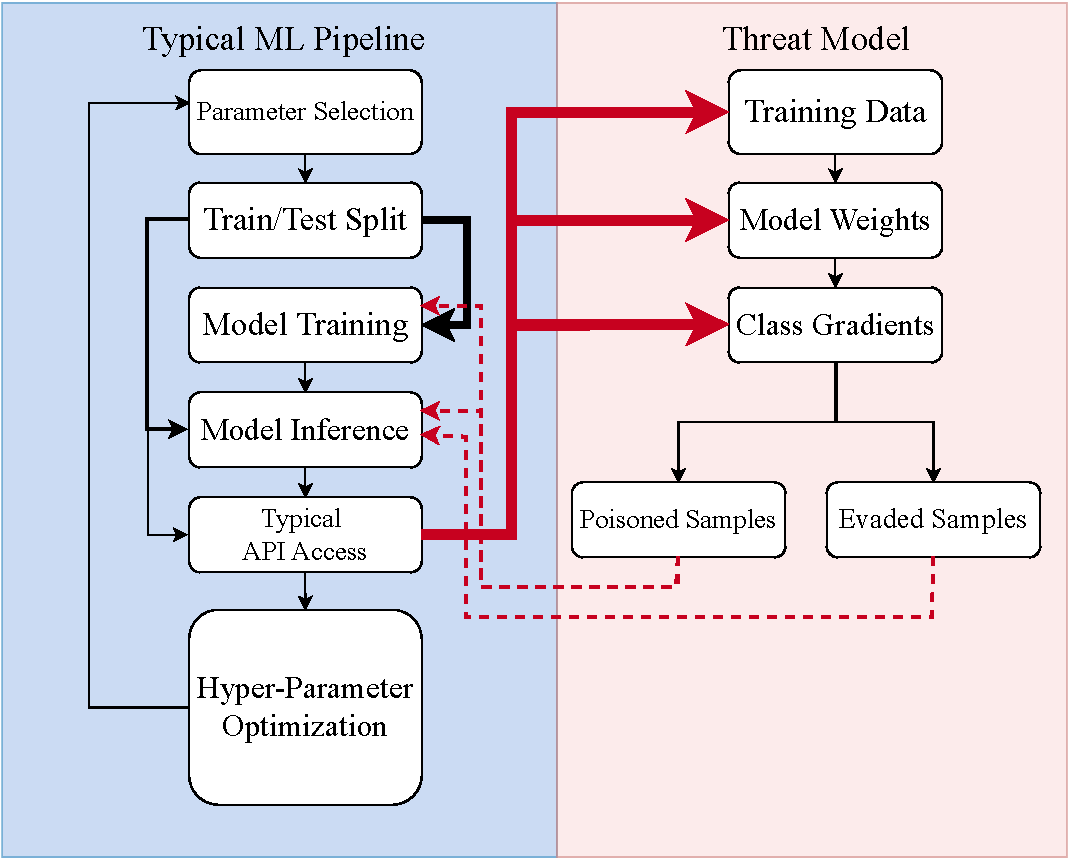
\includegraphics[width=.8\textwidth]{images/attack_diagram.pdf}
    \caption{This diagram depicts the various threat models against a typical machine learning model.}
    \label{fig:threat_model}
\end{figure*}
\label{threat}

\subsection{Attacks}
\label{attacks}
\begin{itemize}
    \item FGM
    \item HSJ


\end{itemize}
\subsubsection{Attack Related Metrics}
\paragraph{Minimal Evasion Distance}
\paragraph{Survival Time}
% \pargraph{KL_Divergence}
\paragraph{SHAPr Privacy Metric}
\section{Improving GZIP-KNN}
\label{improvements}
We can use this model in two different paradigms. In general, the idea is that the number of requisite training samples is very small, so we can run everything client-side, keeping the particulars of the model training private. Another method for distributing the training process, federated learning, trains a model for each user but routinely shares model weights upstream to create a better model for everyone. However, as we outlined in Sec.~\ref{threat}, that opens new attack vectors that would be unsuitable for information the user would like to keep private (\textit{e.g.}, IP address, message contents, or schedule of use). Instead, we propose training a model for each user in one of two scenarios.
\label{improvements}
\subsection{Real-time, time-variant signal processing}
In some situations, it might be necessary to find anomalies in real-time, which involves special considerations. Namely, we can skip the "training" step entirely and select a number of existing samples from our database for training. These could be selected randomly or according to some time filter in an attempt to only capture new or otherwise unnoticed anomalies. In some cases, it may be that the user doesn't have many samples. However, as we show in the Sec.~\ref{results}, that even small training sets are remarkably effective for this method.

\subsubsection{Different measures of distance}
There are many different distance measures. For example we can use normal scikit-learn implementations \footnote{
https://scikit-learn.org/stable/modules/classes.html\#module-sklearn.metrics.pairwise or https://scikit-learn.org/stable/modules/generated/} or just kernel metrics\footnote{sklearn.metrics.pairwise.kernel\_metrics.html\#sklearn.metrics.pairwise.kernel\_metrics}--- both of which are highly parallelizable for single- or multi-core jobs. Let's start with:
\begin{itemize}
    \item $\ell_0$ (bit-wise distance)
    \item $\ell_1$ (taxi-driver distance)
    \item $\ell_2$ (euclidean)
    \item $\mathscr{\chi}^2$ (weighted difference per entry)
    \item $\mathscr{L}$ (Laplacian)
    \item $\mathscr{W}$ (Wasserstein)
\end{itemize}

\subsubsection{Calculating distance matrix}

\subsubsection{Removing time-variant noise using autocorellation techniques}

TODO: talk about arima models


\subsubsection{Pre-computing the Compression vector}
Since the compression step requires the most processing time, we can pre-compute the compression distance for our input data as part of a training step, if we so choose. This offers marginal run-time improvements over the original implementation that repeatedly calculated the NCD of all training samples for each example in the test set.

\subsection{Big data Anomaly Detection}
In other situations, it is necessary to minimize the number of samples used for evaluation because the size of the user's database is too large to evaluated in a reasonable amount of time.








\subsubsection{Reducing the Search Space}
We can use a variety of algorithms to reduce the size of our search space. 
\begin{itemize}
    \item Mean Distance
    \item Medoid
    \item Random
    \item KNN
    \item SVC
\end{itemize}


\begin{algorithm}
  \caption{Find M-Best Indices}
  \SetAlgoNlRelativeSize{0}
  \SetAlgoNlRelativeSize{-1}
  \SetAlgoNlRelativeSize{-2}
  
  \KwData{Sample points $P$, Number of best indices $m$}
  \KwResult{Set of indices $I$ with the m-best points}
  
  \ForEach{point $p$ in $P$}{
    Calculate a relevance score $r_p$ based on some criterion\;
  }
  
  Sort indices based on relevance scores in descending order: $I \gets$ sortIndices($r_p$)\;
  
  \Return top $m$ indices $I$\;
\end{algorithm}



\subsubsection{Iterative Methods}
We can now treat this as an iterative problem and do a continuous hyperparameter search.


\begin{algorithm}
    \caption{Sample Points}
    \KwData{Training samples, $X$; and their labels, $y$}
    \KwResult{Training samples, $X_{train}$ and their labels, $y_{train}$}
\end{algorithm}

\begin{algorithm}
  \caption{Model Training}
  
  \KwData{System state $S$, Number of iterations $N$, Number of best indices $m$, $x_{test}, y_{test}, X_{train}, y_{train}$}
  \KwResult{Final system state $S$}
  
  Initialize system: $S \gets$ baseline state\;
  \For{$i=1$ to $N$}{
    Sample points: $P \gets$ samplePoints($S$)\;
    Find m-best indices: $I \gets$ findMBestIndices($P, m$)\;
  }
  \Return $m$-best indices, $I$\;
\end{algorithm}







\section{Methods}

\subsection{Datasets}
\begin{itemize}
    \item KDD-NSL (Intrusion Detection)
    \item Truthseeker (Twitter Bot)
    \item Email Spam
    \item PCAP DDOS
\end{itemize}
\subsection{Models}

\paragraph{$k$-clusters}
To use KNN, one must specify a number of nearest neighbors to use for class prediction (see: Algorithm~\ref{alg:knn})
\paragraph{Compressors:} In addition to \texttt{gzip}, we tried numerous different compression algorithms. 
\begin{itemize}
    \item gzip - widely available, fast compared to lzma/bz2
    \item lzma - more compression, more time
    \item bz2 - balances gzip/bz2
    \item zstd - designed around real-time usage at the expense of compression depth
\end{itemize}

\paragraph{Training Sample Optimization:}
We provide theoretical justifications for using secondary methods for determining ideal training set in Section~\ref{improvements}. For the sake of completeness, we tested the mean, medoid, random, KNN, and SVC methods outlined above as well as selecting the $m$-most important samples for each with $m \in$ [10,20,50,100,200,500,1000]. 
\begin{itemize}
    \item Mean Distance
    \item Medoid
    \item Random
    \item KNN
    \item SVC
\end{itemize}

\subsection{Metrics}
\label{metrics}
\label{methods}
\section{Results}

\subsection{Accuracy}

\begin{figure*}
	\begin{subfigure}
		\centering
		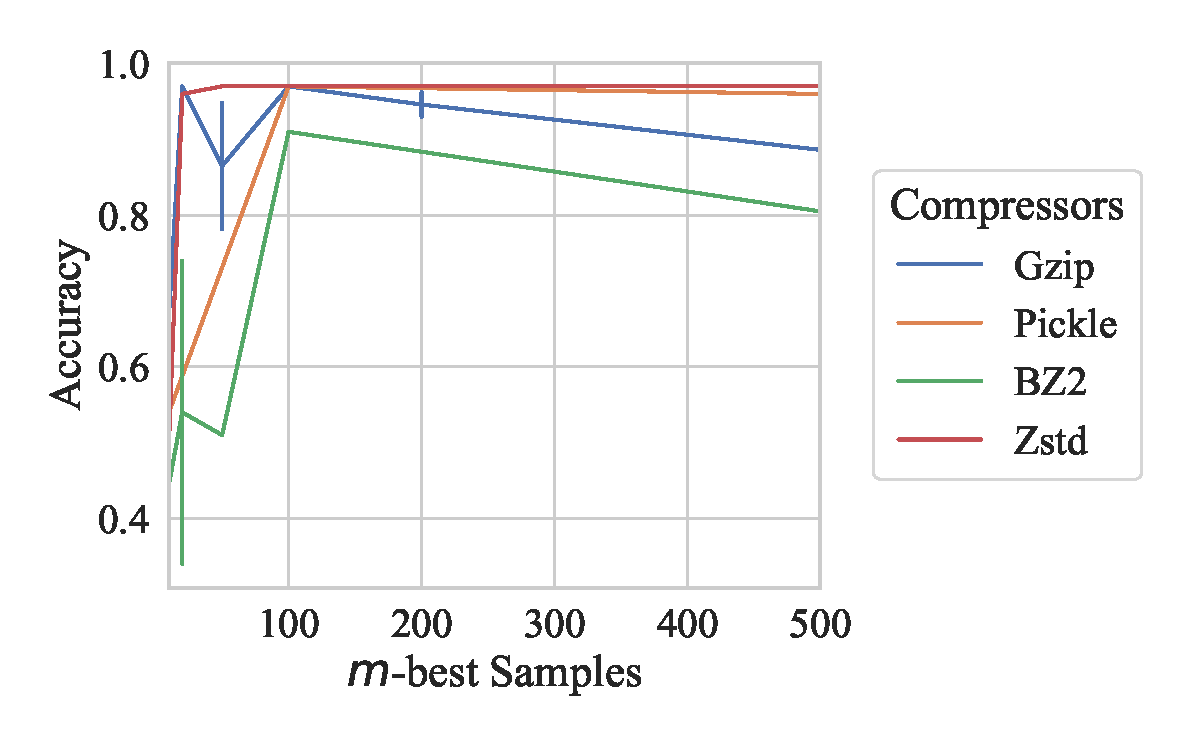
\includegraphics[width=.32\textwidth]{figs/truthseeker/compressor_vs_accuracy.pdf}
	\end{subfigure}%
	~
	\begin{subfigure}
		\centering
		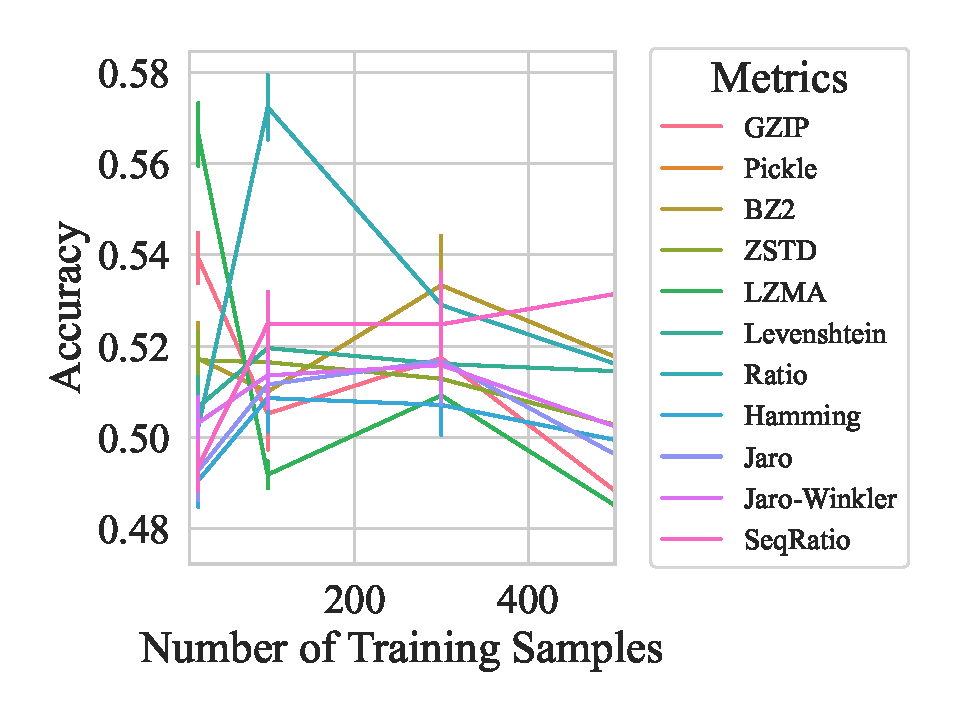
\includegraphics[width=.32\textwidth]{figs/truthseeker/metric_vs_accuracy.pdf}
	\end{subfigure}
	~
	\begin{subfigure}
		\centering
		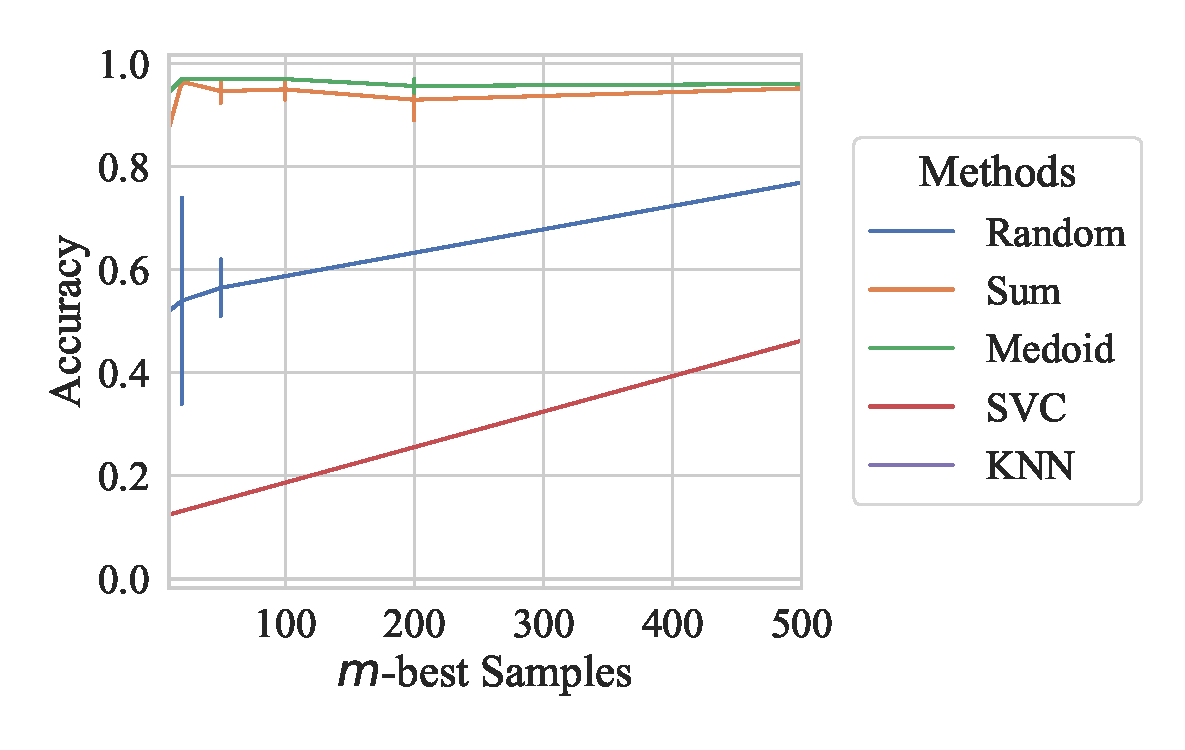
\includegraphics[width=.32\textwidth]{figs/truthseeker/method_vs_accuracy.pdf}
	\end{subfigure}
	\caption{ Caption...}.
	\label{fig:accuracy}
\end{figure*}

\subsection{Training Time}

\begin{figure*}
	\begin{subfigure}
		\centering
		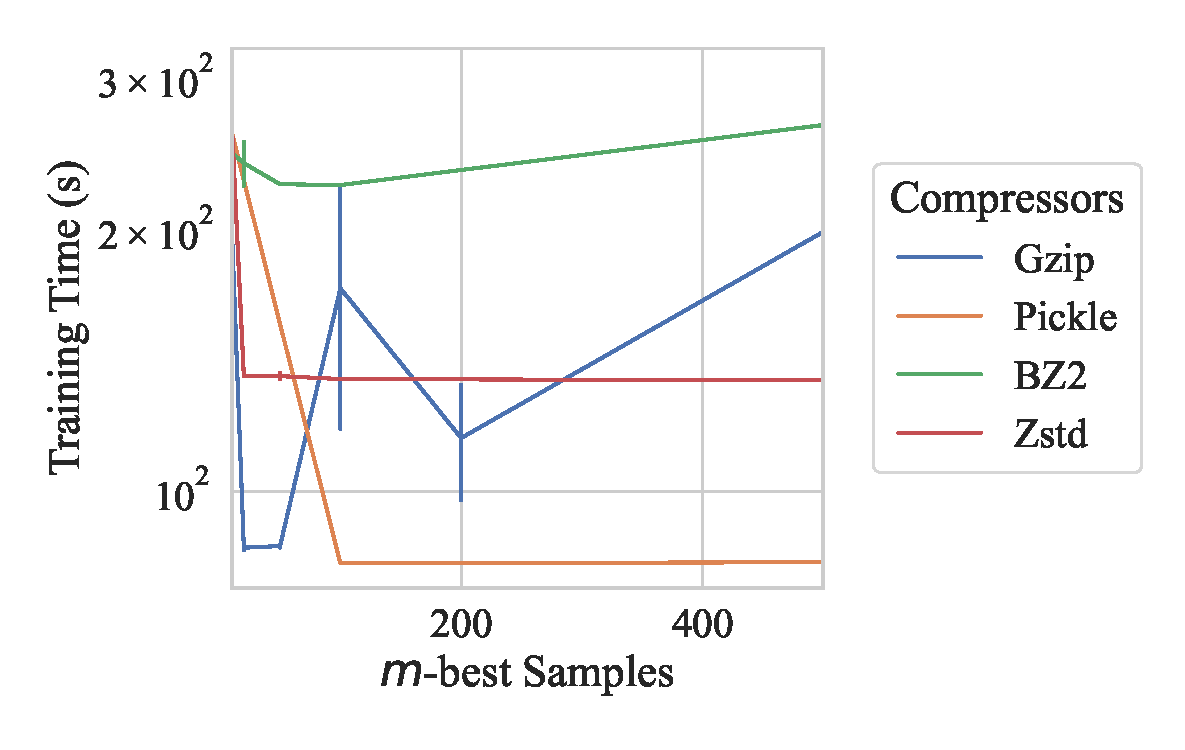
\includegraphics[width=.32\textwidth]{figs/truthseeker/compressor_vs_train_time.pdf}
	\end{subfigure}%
	~
	\begin{subfigure}
		\centering
		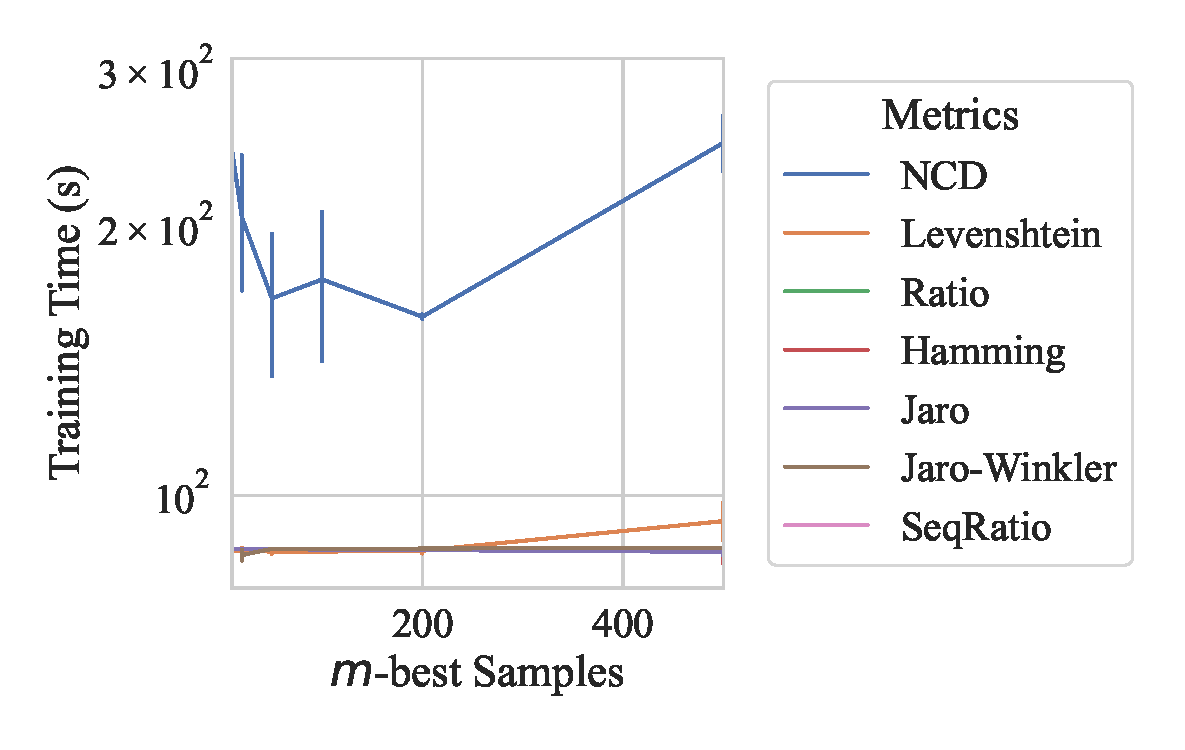
\includegraphics[width=.32\textwidth]{figs/truthseeker/metric_vs_train_time.pdf}
	\end{subfigure}
	~
	\begin{subfigure}
		\centering
		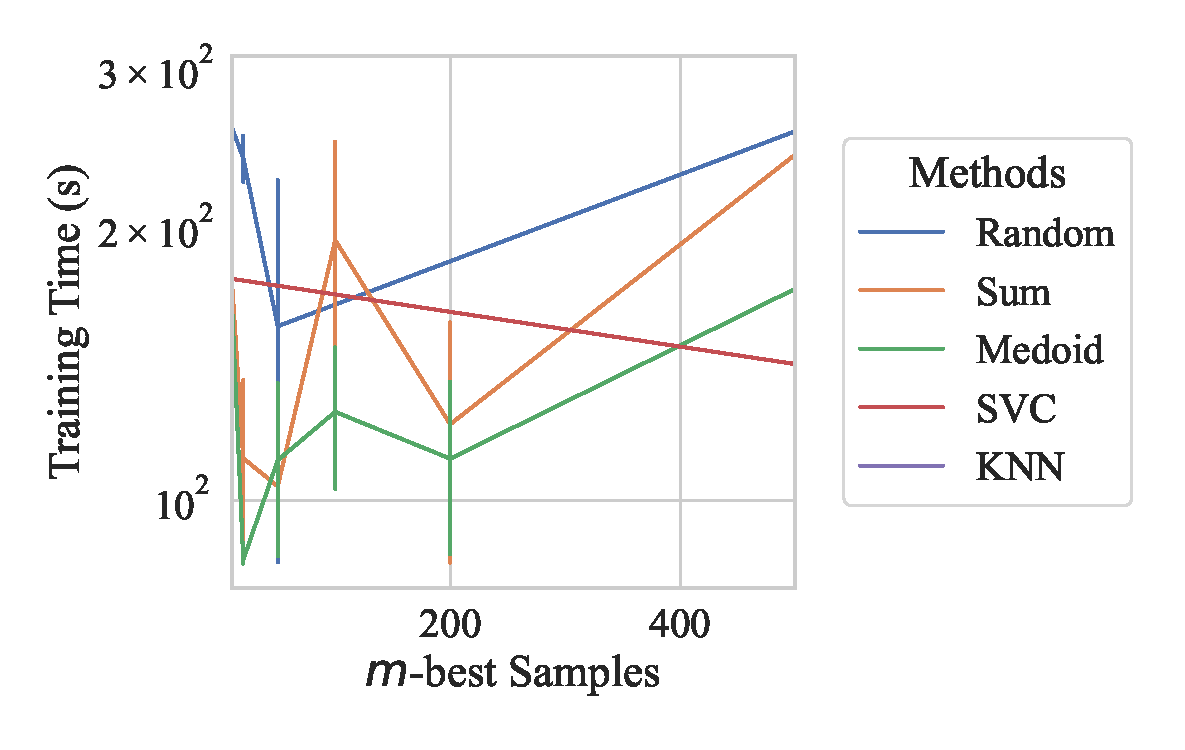
\includegraphics[width=.32\textwidth]{figs/truthseeker/method_vs_train_time.pdf}
	\end{subfigure}
	\caption{ Caption...}.
	\label{fig:accuracy}
\end{figure*}

\subsection{Prediction Time}


\begin{figure*}
	\begin{subfigure}
		\centering
		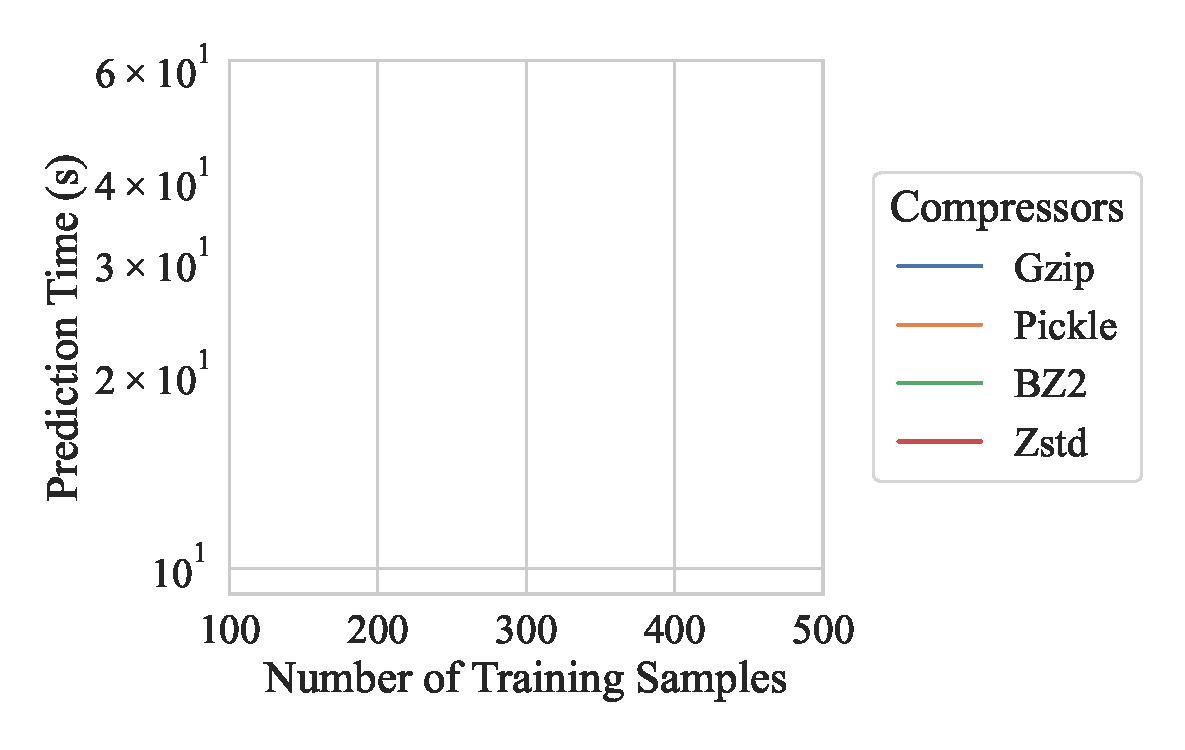
\includegraphics[width=.32\textwidth]{figs/truthseeker/compressor_vs_predict_time.pdf}
	\end{subfigure}%
	~
	\begin{subfigure}
		\centering
		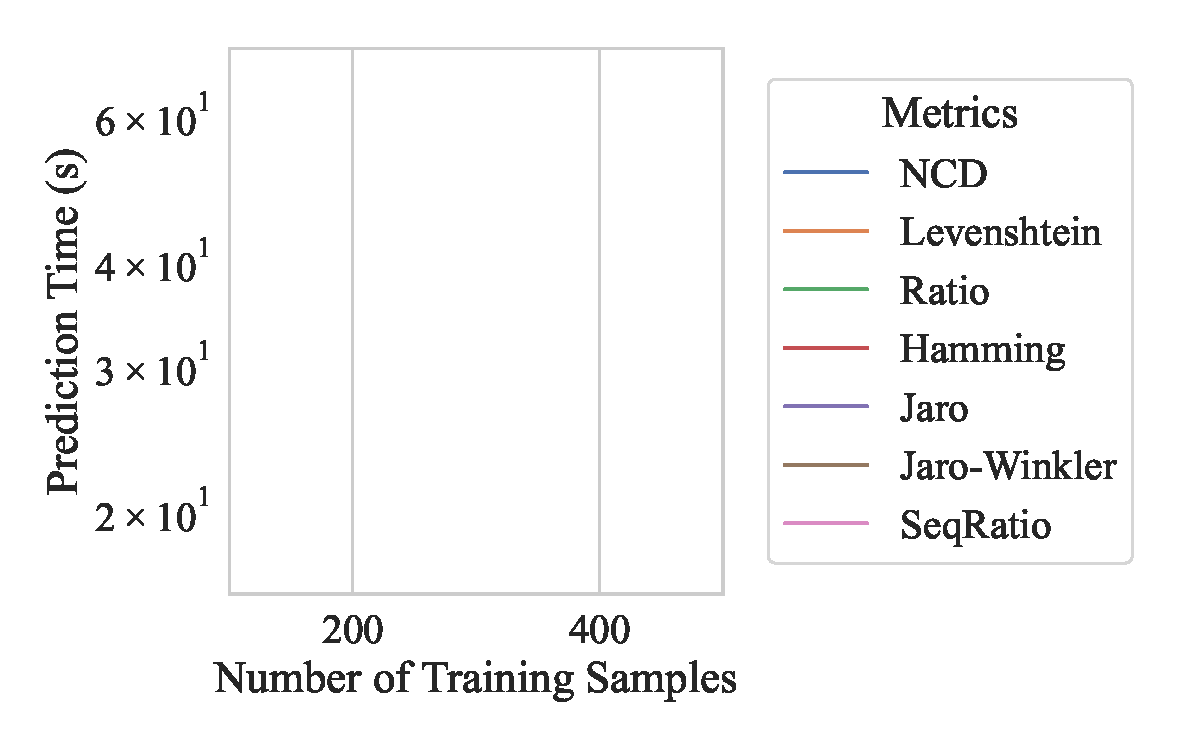
\includegraphics[width=.32\textwidth]{figs/truthseeker/metric_vs_predict_time.pdf}
	\end{subfigure}
	~
	\begin{subfigure}
		\centering
		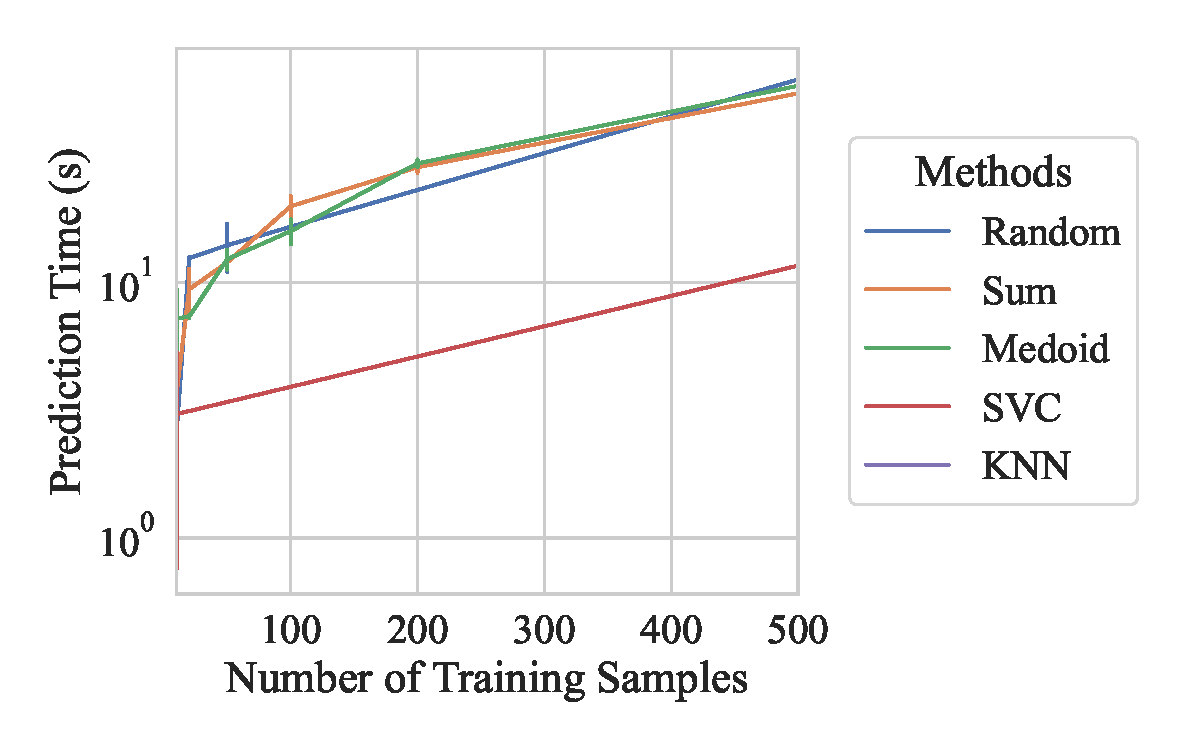
\includegraphics[width=.32\textwidth]{figs/truthseeker/method_vs_predict_time.pdf}
	\end{subfigure}
	\caption{ Caption...}.
	\label{fig:accuracy}
\end{figure*}

\subsection{Symmetry}



\label{results}
\section{Considerations}
\label{considerations}
\section{Conclusion}
\label{conclusion}


\end{document}
\endinput
%%
